\documentclass[main.tex]{subfiles}
\begin{document}

\chapter{Logic Diagrams}

\section{Simple wrapping}
\begin{figure}[h]
    \centering
    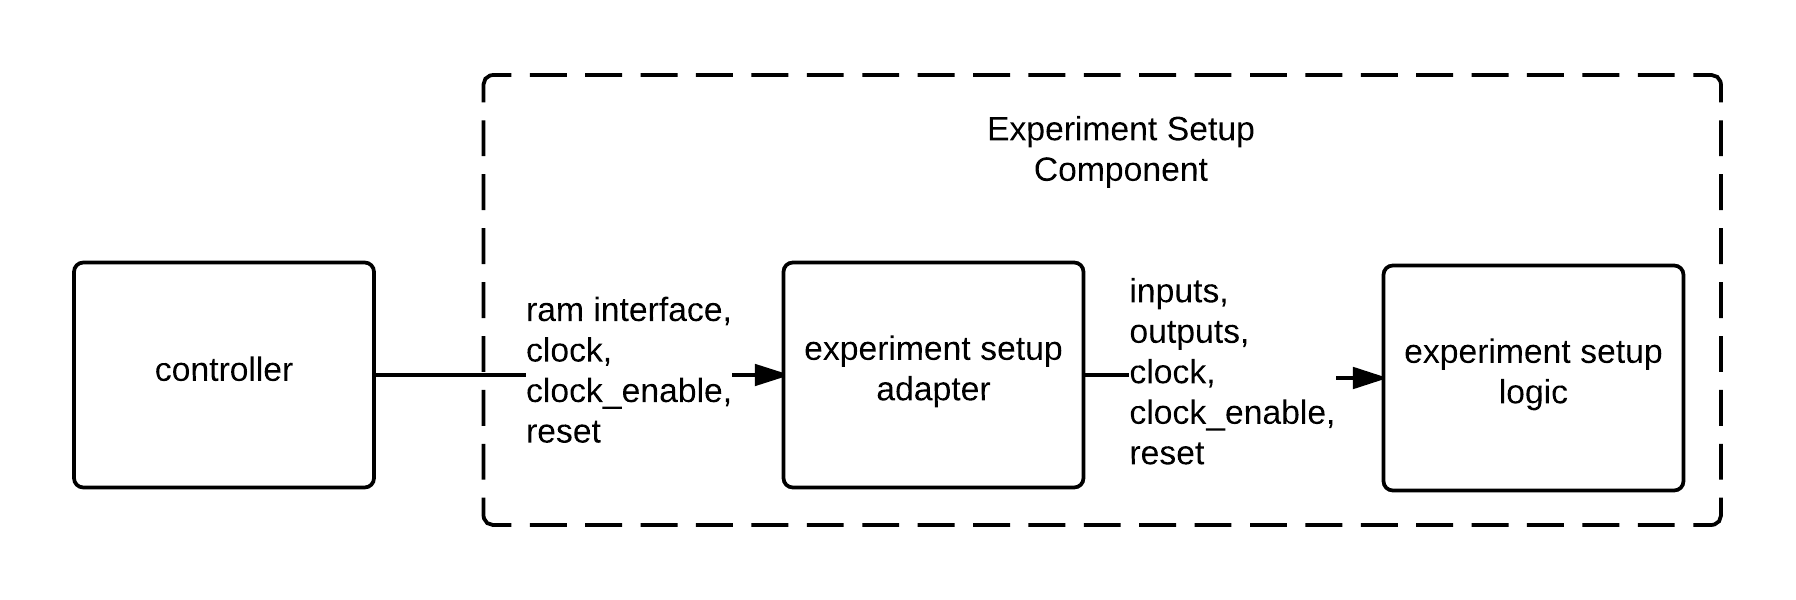
\includegraphics[width=\textwidth]{img/logic-wrap-simple}
    \caption{Caption}
    \label{fig:logic-wrap-simple}
\end{figure}

\begin{landscape}
    \section{Advanced wrapping}
    \begin{figure}[h]
        \centering
        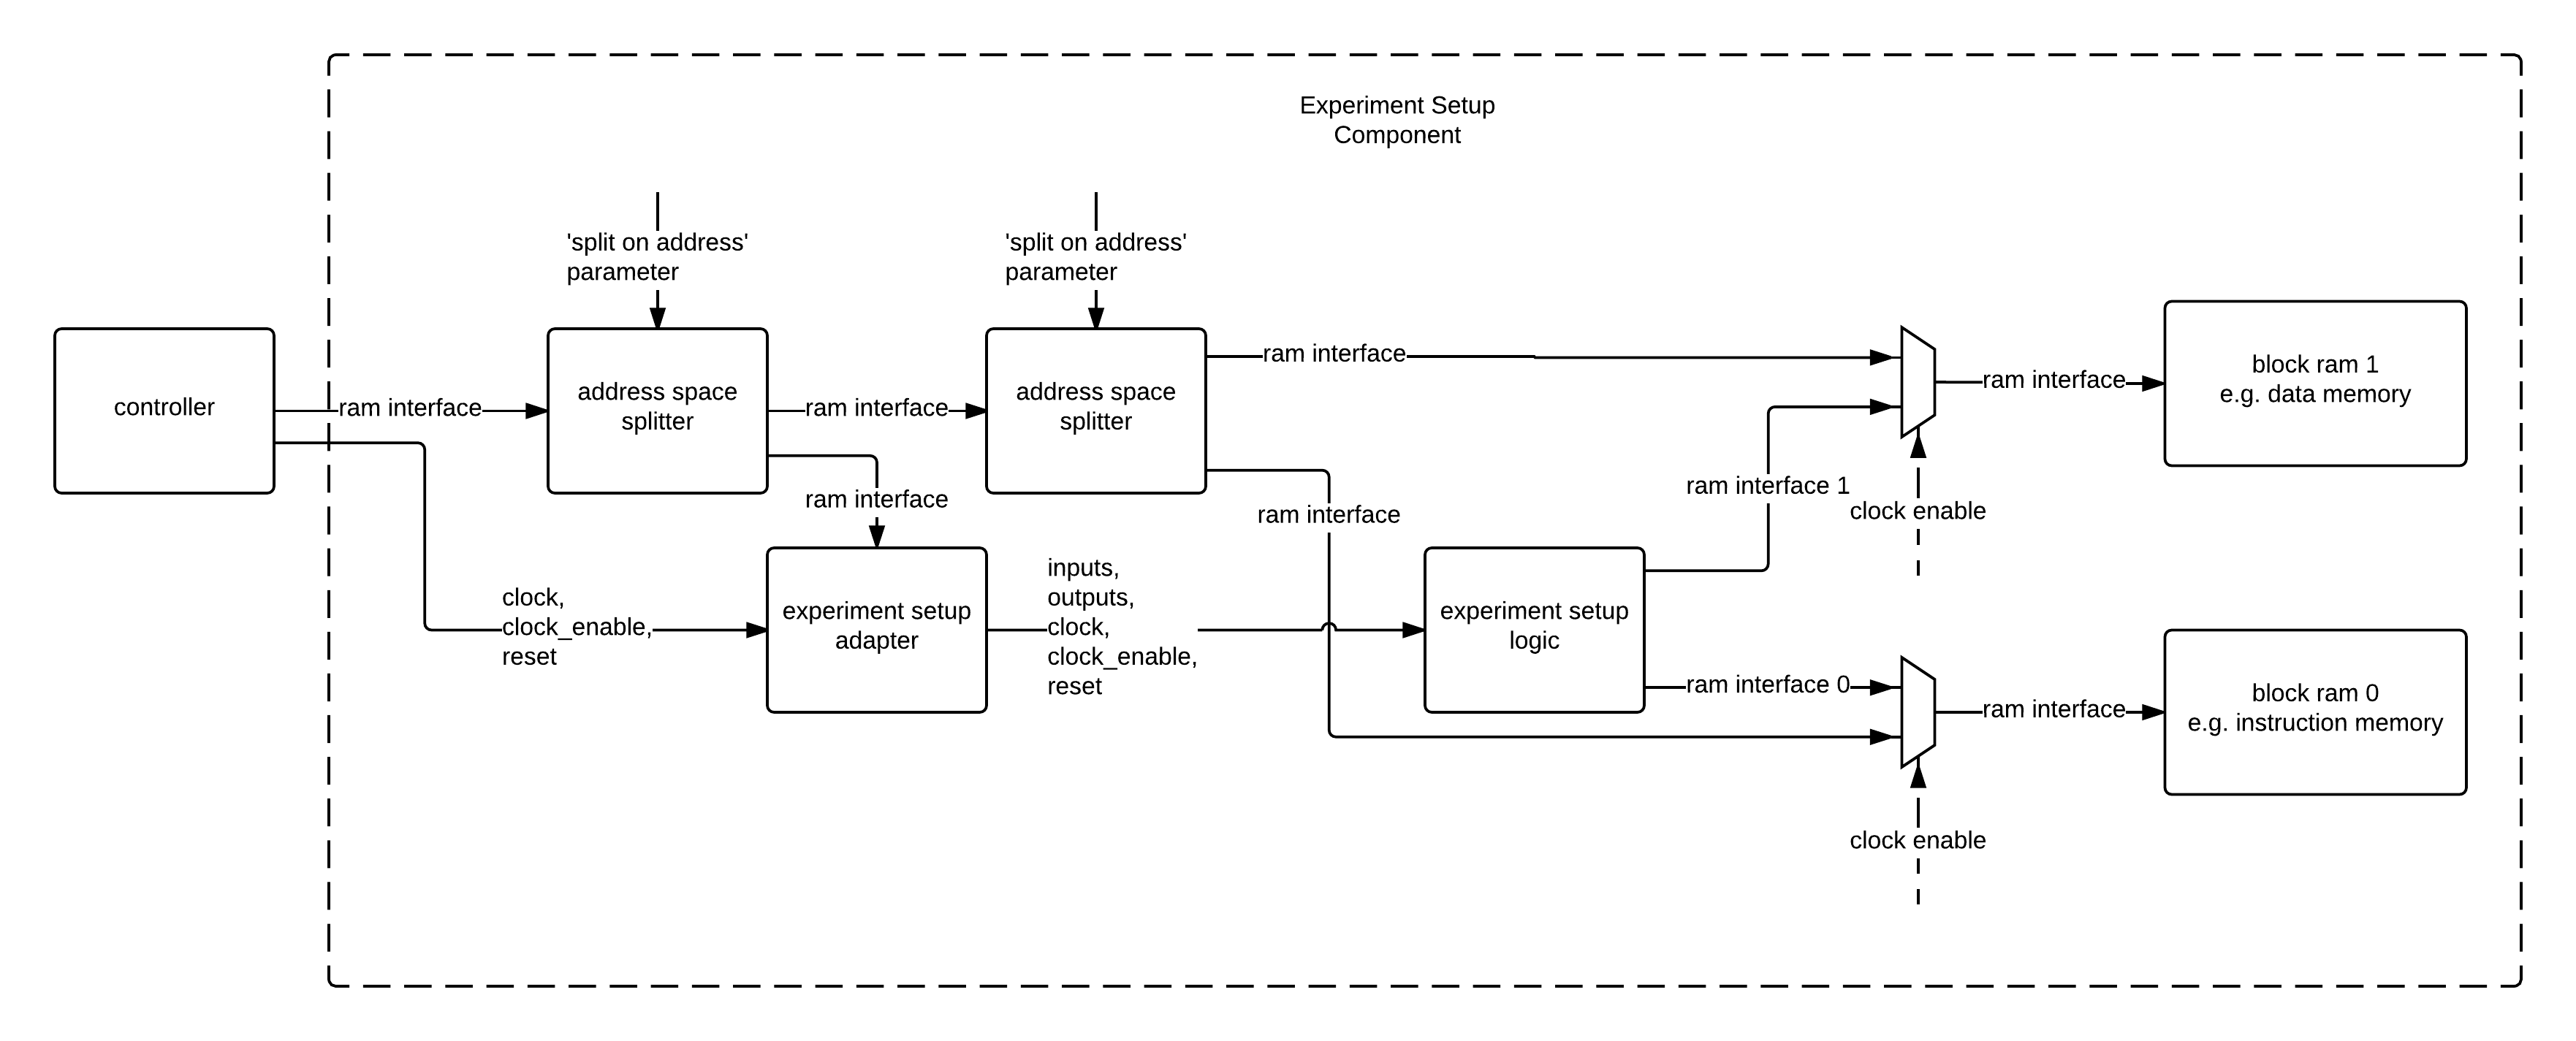
\includegraphics[width=\hsize]{img/logic-wrap-extended}
        \caption{Complex wrapper}
        \label{fig:logic-wrap-extended}
    \end{figure}
\end{landscape}

\section{Experiment Adapter}
\begin{figure}[h]
    \centering
    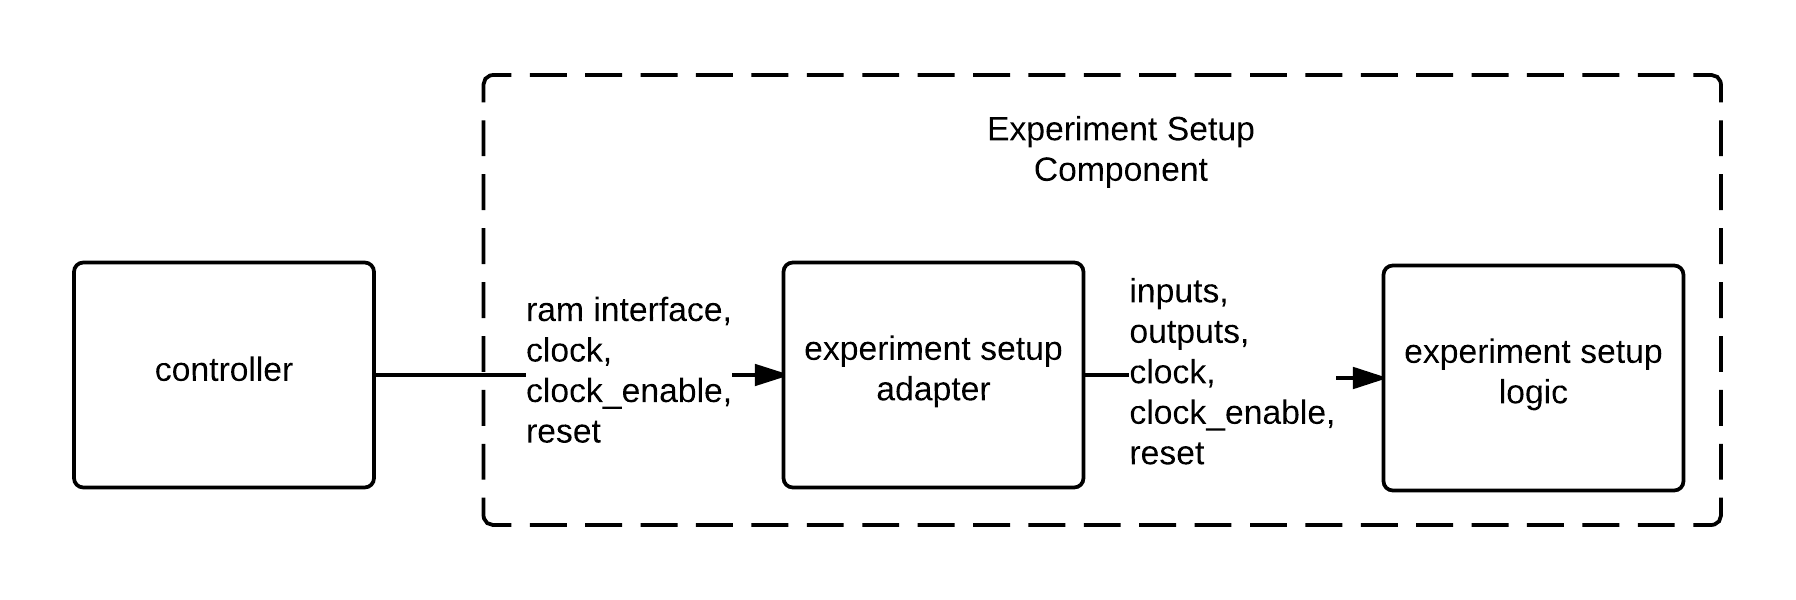
\includegraphics[width=\textwidth]{img/logic-wrap-simple}
    \caption{Caption}
    \label{fig:logic-experiment-adapter}
\end{figure}

\end{document}